\documentclass[tikz,border=10pt]{standalone}
\usepackage{tikz}
\usetikzlibrary{angles,quotes,calc, arrows.meta, intersections}

\begin{document}
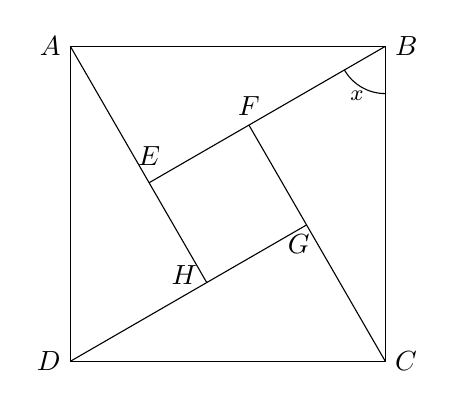
\begin{tikzpicture}

% Draw a square
\coordinate (A) at (0,4);
\coordinate (B) at (4,4);
\coordinate (C) at (4,0);
\coordinate (D) at (0,0);
\draw (A)  -- (B) -- (C) -- (D) -- cycle;

%label vertices
\node at (A) [anchor = east] {$A$};
\node at (B) [anchor = west] {$B$};
\node at (C) [anchor = west] {$C$};
\node at (D) [anchor = east] {$D$};

\path[name path=leg1] (A) -- ($(A)!1!30:(D)$) coordinate (N);
\path[name path=leg2] (D) -- ($(D)!1!30:(C)$) coordinate (O);
\path[name path=leg3] (C) -- ($(C)!1!30:(B)$) coordinate (P);
\path[name path=leg4] (B) -- ($(B)!1!30:(A)$) coordinate (Q);

\draw[name intersections={of=leg1 and leg2,by={H}}] (A) -- (H);
\draw[name intersections={of=leg3 and leg2,by={G}}] (D) -- (G);
\draw[name intersections={of=leg3 and leg4,by={F}}] (C) -- (F);
\draw[name intersections={of=leg4 and leg1,by={E}}] (B) -- (E);

\node at (E) [anchor = south, yshift = 0.1cm] {$E$};
\node at (F) [anchor = south] {$F$};
\node at (G) [anchor = north, xshift = -0.1cm] {$G$};
\node at (H) [anchor = east, yshift = 0.1cm] {$H$};

\pic [draw, "\footnotesize $x$ ", angle eccentricity=1.2, angle radius=0.6cm] {angle = F--B--C};


\end{tikzpicture}
\end{document}
